\section{Konjunktur}
\subsection{Der negative Nachfrageschock}
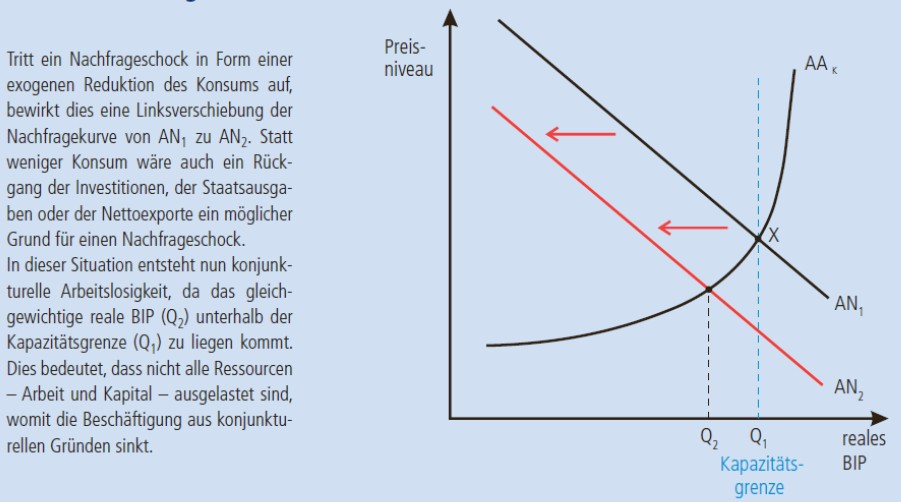
\includegraphics[width=0.8\linewidth]{images/negnach.jpg}
\begin{multicols}{2}
\subsection{Der kurzfristige positive Nachfrageschock}
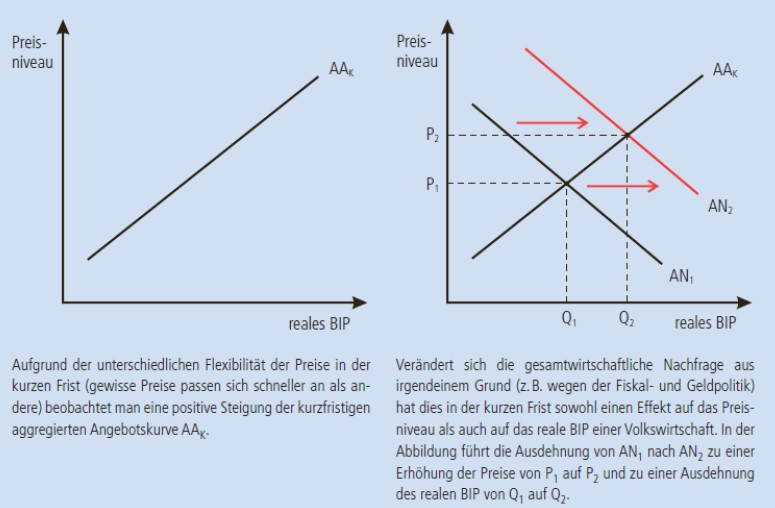
\includegraphics[width=0.98\linewidth]{images/posnachkurz.jpg}
\subsection{Der langfristige positive Nachfrageschock}
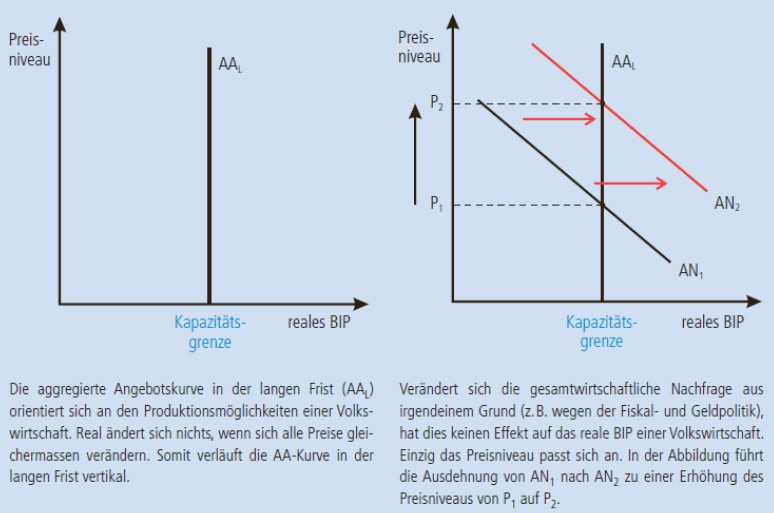
\includegraphics[width=0.98\linewidth]{images/posnachlang.jpg}
\end{multicols}
\begin{multicols}{2}
\subsection{Der negative Angebotsschock}
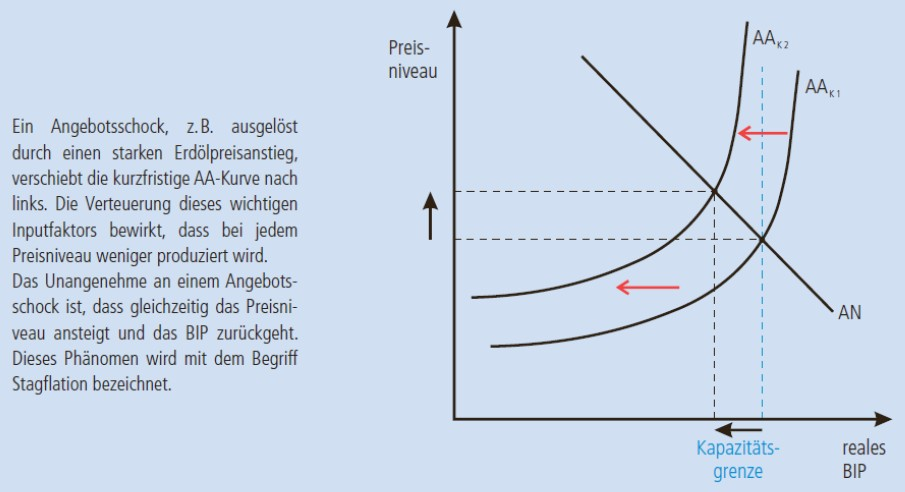
\includegraphics[width=0.98\linewidth]{images/negangebot.jpg}
\subsection{Der positive Angebotsschock}
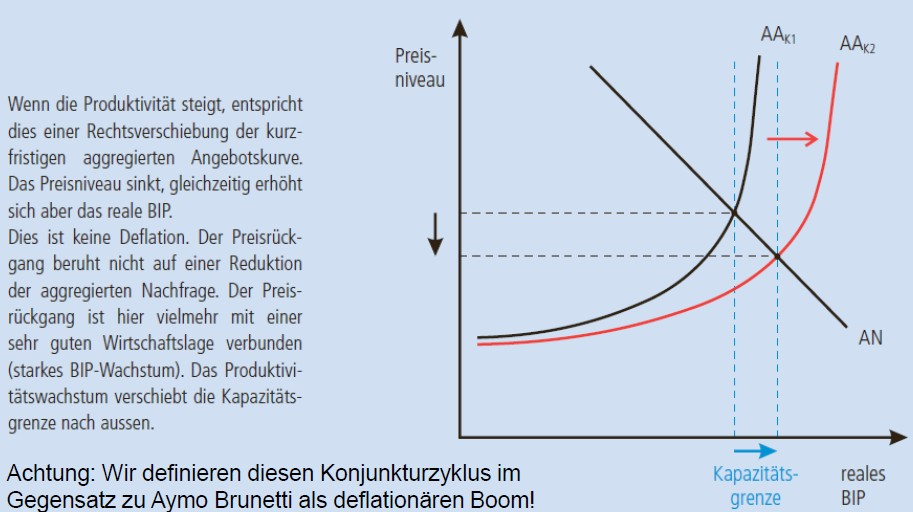
\includegraphics[width=0.98\linewidth]{images/posangebot.jpg}
\end{multicols}
\subsection{Konjunkturzyklen}
	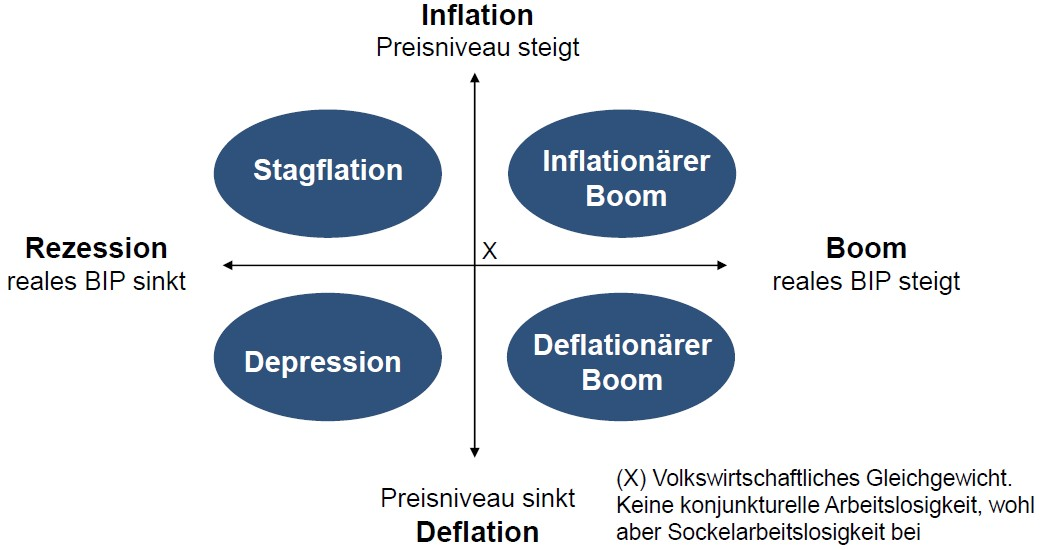
\includegraphics[width=15cm]{images/konjukturzyklen.jpg}\\
\begin{minipage}{10cm}
	\begin{itemize}
		\item \textbf{1.Nichts tun} 
		\subitem Anpassung ohne aktive Konjunkturpolitik
		\subitem Automatisches Wiederherstellen auf lange Sicht
		\subitem Zuerst Sinken der Löhne (Nominallöhne)
		\subitem Anschliessend tiefere Lohnkosten für Unternehmen dadurch höheres Angebot
		\subitem Gleiches BIP aber tieferes Preisniveau, tiefere Nominallöhne	
	\end{itemize}
\end{minipage}
\begin{minipage}{9cm}
	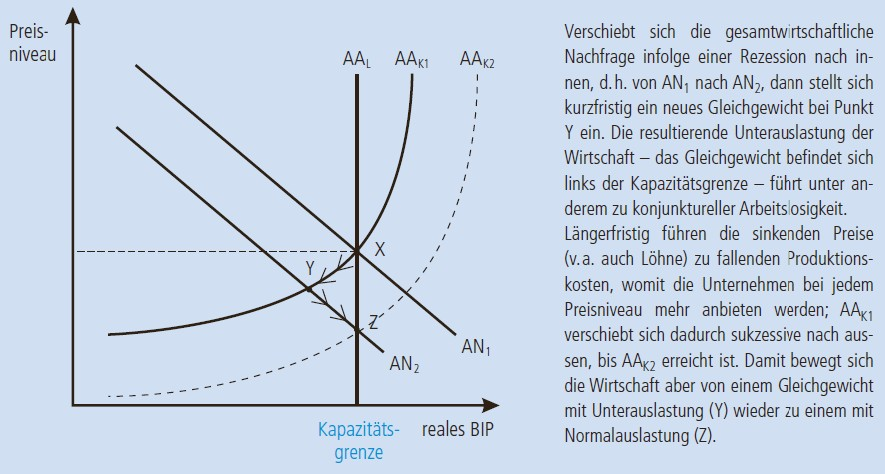
\includegraphics[width=9cm]{images/nichts.jpg}
\end{minipage}
\begin{minipage}{10cm}
	\begin{itemize}
		\item \textbf{2.Aktive keynesianische Konjukturpolitik}
		\subitem Märkte gehen von selbst, aber langsam wieder ins Gleichgewicht
		\subitem Positiver Schock auf Nachfrageseite
		\subitem Staat fördert durch Fiskal- und Geldpolitik Konsumnachfrage
		\subitem Staat erhöht Ausgaben
		\subitem Stimulierung der Investitionsnachfrage der Unternehmen durch tiefe Zinsen
		\subitem Erhöhung der Nettoexporte durch schwächere Währung (Erhöhung der Geldmenge)
		\subitem Problem der Wirkungsverzögerung
	\end{itemize}
\end{minipage}
\begin{minipage}{9cm}
	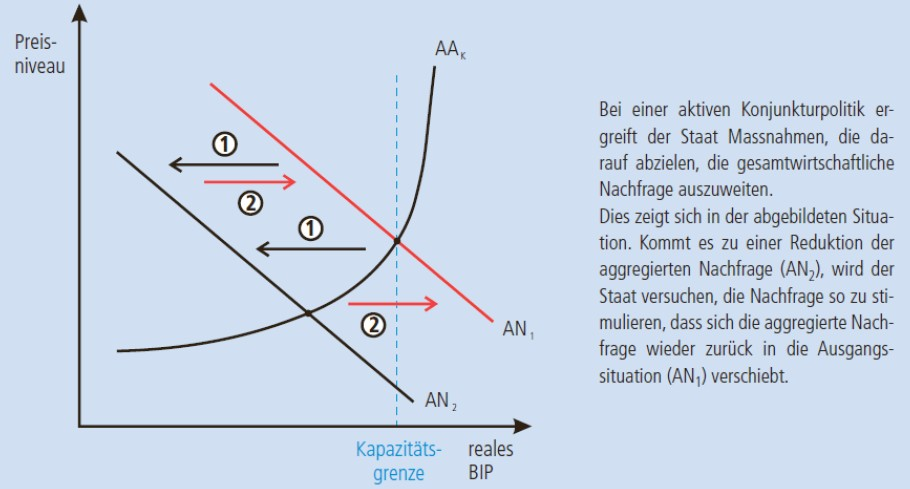
\includegraphics[width=9cm]{images/keyne.jpg}
\end{minipage}
\begin{minipage}{10cm}
	\begin{itemize}
		\item \textbf{3.Stärkung automatische Stabilisatoren}
		\subitem Staatliche Einnahmen und Ausgaben, dass automatisch Nachfrage stimuliert werden
		\subitem Steuern, Schuldenbremse, Arbeitslosenversicherung
	\end{itemize}
\end{minipage}
\begin{minipage}{9cm}
	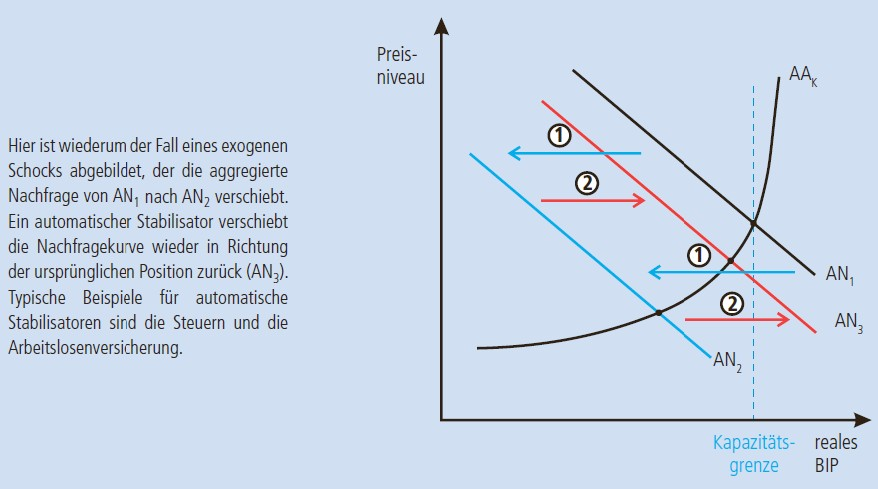
\includegraphics[width=9cm]{images/autostab.jpg}
\end{minipage}
\clearpage
